% Section to be included in the main paper
% Depends on: booktabs, graphicx packages

\subsection{Layer~2 Attention Depends Exclusively on MLP1 Output}
\label{sec:attn2-mlp1-dependence}

A central structural property of the leap-former sorting circuit is that the
query--key matching in the second attention layer (attn2) depends almost
exclusively on the output of the first-layer MLP (MLP1), and not on the other
components of the residual stream---namely the raw token+positional embeddings
and the first-layer attention output (attn1).

\paragraph{Measurement.}
To quantify this, we compare the full attn2 attention distribution
$\mathbf{p}_{\text{normal}}$ (computed from the complete residual stream
$\mathbf{e} + \mathbf{a}_1 + \mathbf{m}_1$) with the distribution
$\mathbf{p}_{\text{mlp1-only}}$ (computed from the residual containing only
$\mathbf{m}_1$, with both $\mathbf{e}$ and $\mathbf{a}_1$ zeroed out). For
each query position in the sorted output region, we compute the $\ell_1$
distance:
\[
  d = \sum_{j} \bigl| p_{\text{normal}}(j) - p_{\text{mlp1-only}}(j) \bigr|,
\]
which ranges from~$0$ (identical distributions) to~$2$ (disjoint support).

\paragraph{Results across leap-former checkpoints.}
We evaluate this metric on all 15 leap-former checkpoints identified across our
training grid (8~configurations $\times$ 5~seeds, classified by whether
removing attn2 reduces full-sequence accuracy to near zero).
Figure~\ref{fig:probl1distance} reports the mean $\ell_1$ distance for each
checkpoint, averaged over ${\geq}225{,}000$ query positions per model.

\begin{figure}[t]
  \centering
  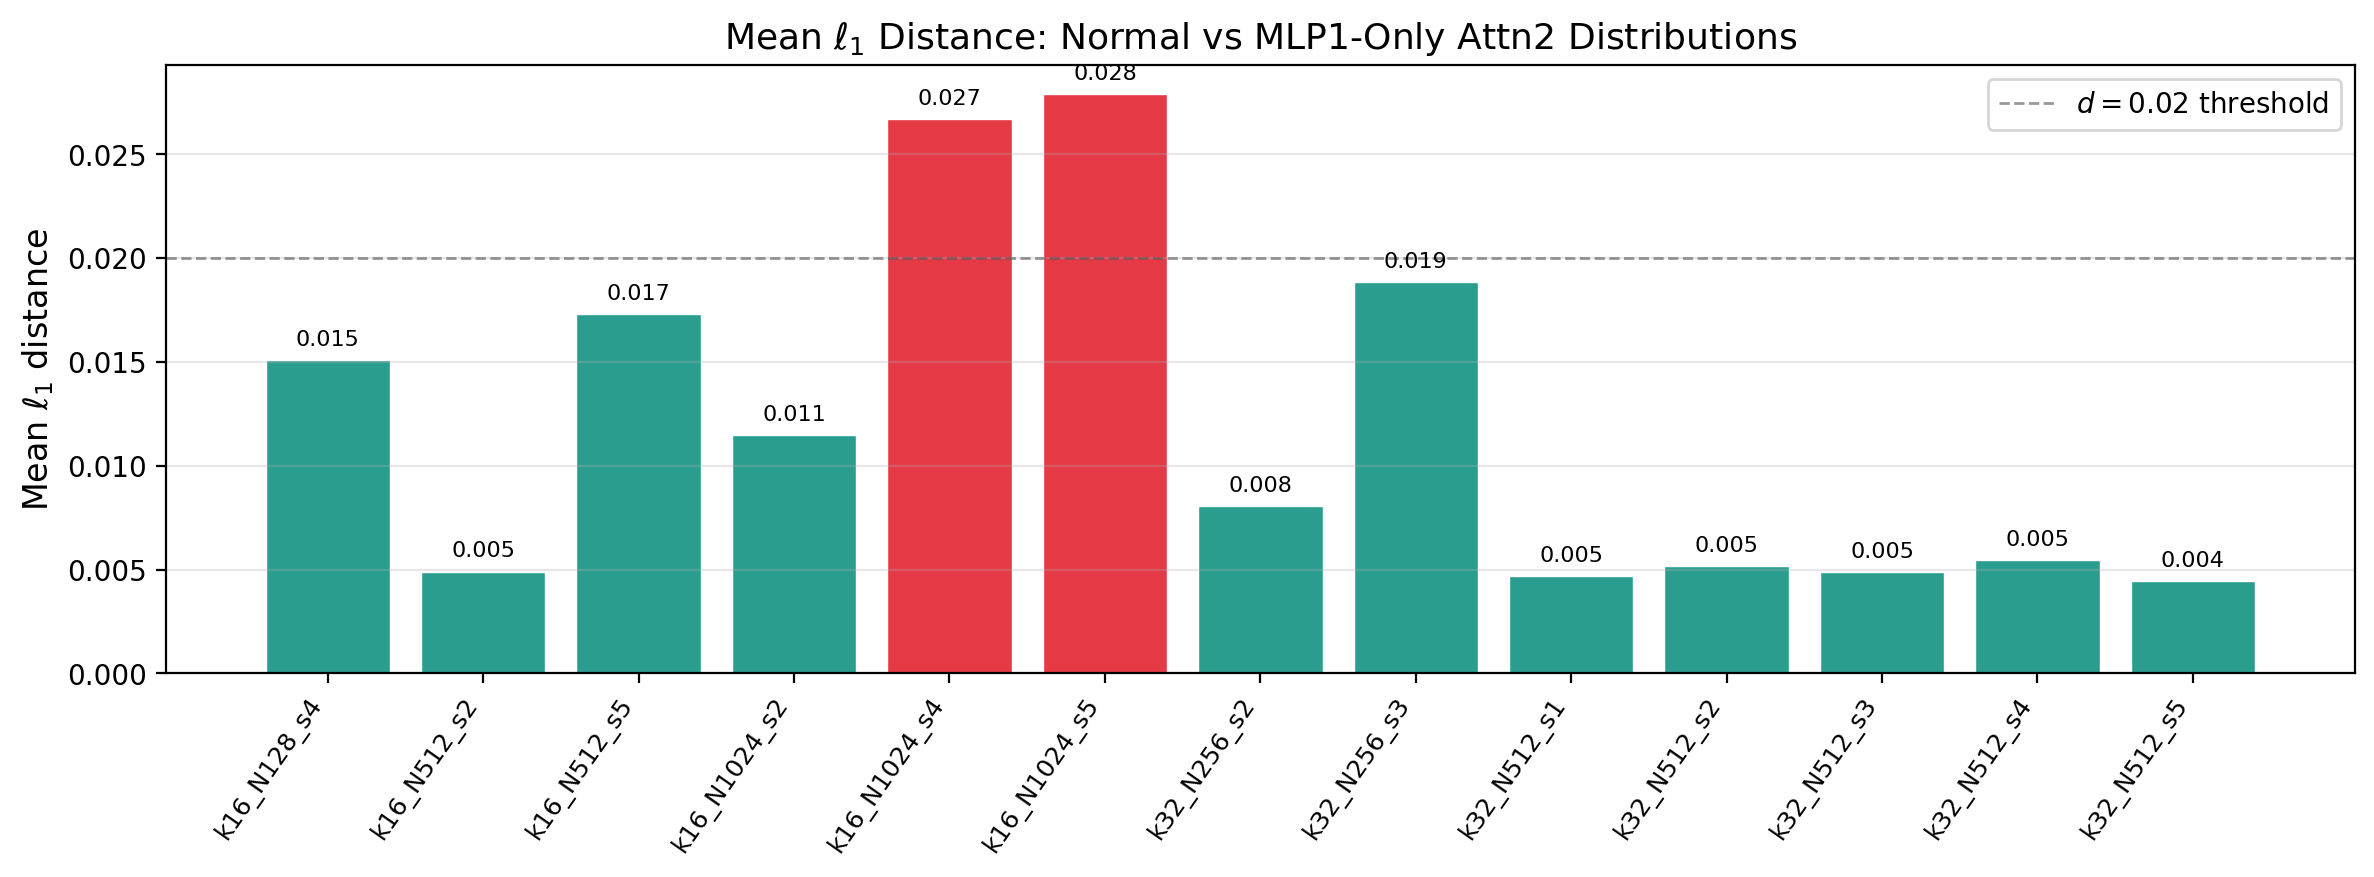
\includegraphics[width=\linewidth]{mechanistic-interpretability/attn2-mlp1-dependence/probl1distance_all_leapformers.png}
  \caption{%
    Mean $\ell_1$ distance between normal and MLP1-only attn2 probability
    distributions across all leap-former checkpoints. Green bars indicate
    models where attn2 depends almost exclusively on MLP1 output
    (mean~$d < 0.02$); red bars indicate outliers with non-trivial dependence
    on other residual stream components. The dashed line marks the $0.02$
    threshold.}
  \label{fig:probl1distance}
\end{figure}

Of the 15~leap-former checkpoints, 12 exhibit mean $\ell_1$
distances below~$0.02$ (median typically below~$0.01$), confirming that attn2's
query--key scores are determined almost entirely by MLP1 output. The effect is
particularly consistent for the \texttt{k32\_N512} configuration: all five
seeds yield mean distances of $0.004$--$0.005$, indicating that this property
is robust to random initialization.

\paragraph{Outliers at large vocabulary size.}
Two checkpoints deviate from this pattern:
\texttt{k16\_N1024\_s3} (mean $d = 0.133$, $p_{99} = 0.99$) and
\texttt{k32\_N1024\_s5} (mean $d = 0.299$, $p_{99} = 2.0$). Both correspond
to the largest vocabulary size ($N = 1024$), suggesting that as the number of
tokens grows, some training runs discover solutions in which attn2 additionally
exploits embedding or attn1 information in the residual stream. Notably, other
seeds at $N = 1024$ (e.g., \texttt{k16\_N1024\_s2} with $d = 0.011$) do
\emph{not} exhibit this behavior, indicating that the phenomenon is
seed-dependent rather than a necessary consequence of large vocabulary size.

\paragraph{Scope of subsequent analysis.}
Since the MLP1-only dependence holds for the large majority of leap-former
checkpoints---including all seeds of the primary configuration
(\texttt{k32\_N512}) analyzed in detail throughout this work---the mechanistic
findings reported in subsequent sections (information flow, hijack experiments,
dual-role architecture) apply to the conventional case. The outlier models at
$N = 1024$ represent an alternative learned strategy that does not reduce the
generality of our claims about the dominant sorting mechanism.
